\documentclass{jsarticle}
\usepackage[dvipdfmx]{graphicx}
\begin{document}

\title{身体動作と筋電量の関係性}
\author{平松亨隆}
\maketitle


\section{目的}
私を含めて人は、体を動かすときに意識的に筋肉の伸縮を考えて体を動かすわけではない。だから、例えば腕を曲げるときに上腕二頭筋をどれくらい収縮させるかなどと考える人はいないだろう。そこで、どのように筋肉を収縮させて運動しているのかということを本レポートの目的とした。

\section{実験方法}
\subsection{運動計測}
下記の図\ref{fig:short}はもっとも腕を曲げた状態、図\ref{fig:long}は最も腕を伸ばした状態の図である。被験者にはこの2つの状態を繰り返す腕の曲げ伸ばし運動を、何も指示を出していない速度と速い速度の2パターンで利き腕を動かしてもらって計測をした。その様子を、モーションキャプチャー(ライブラリ社:MoveTR)用の反射マーカーを肩と肘と手首に貼付してビデオカメラで撮影する。このとき、カメラのフレームレートは1000 fpsである。また筋電センサ(ロジカルプロダクト社)を上腕二頭筋と上腕三頭筋に貼付し、その筋電位を計測した。このとき、筋電センサのサンプリング周波数は200 Hzである。筋電センサのカメラと筋電の開始時間は同期をとり、20秒間計測している。
\begin{figure}[h]
  \begin{minipage}{0.5\hsize}
    \begin{center}
      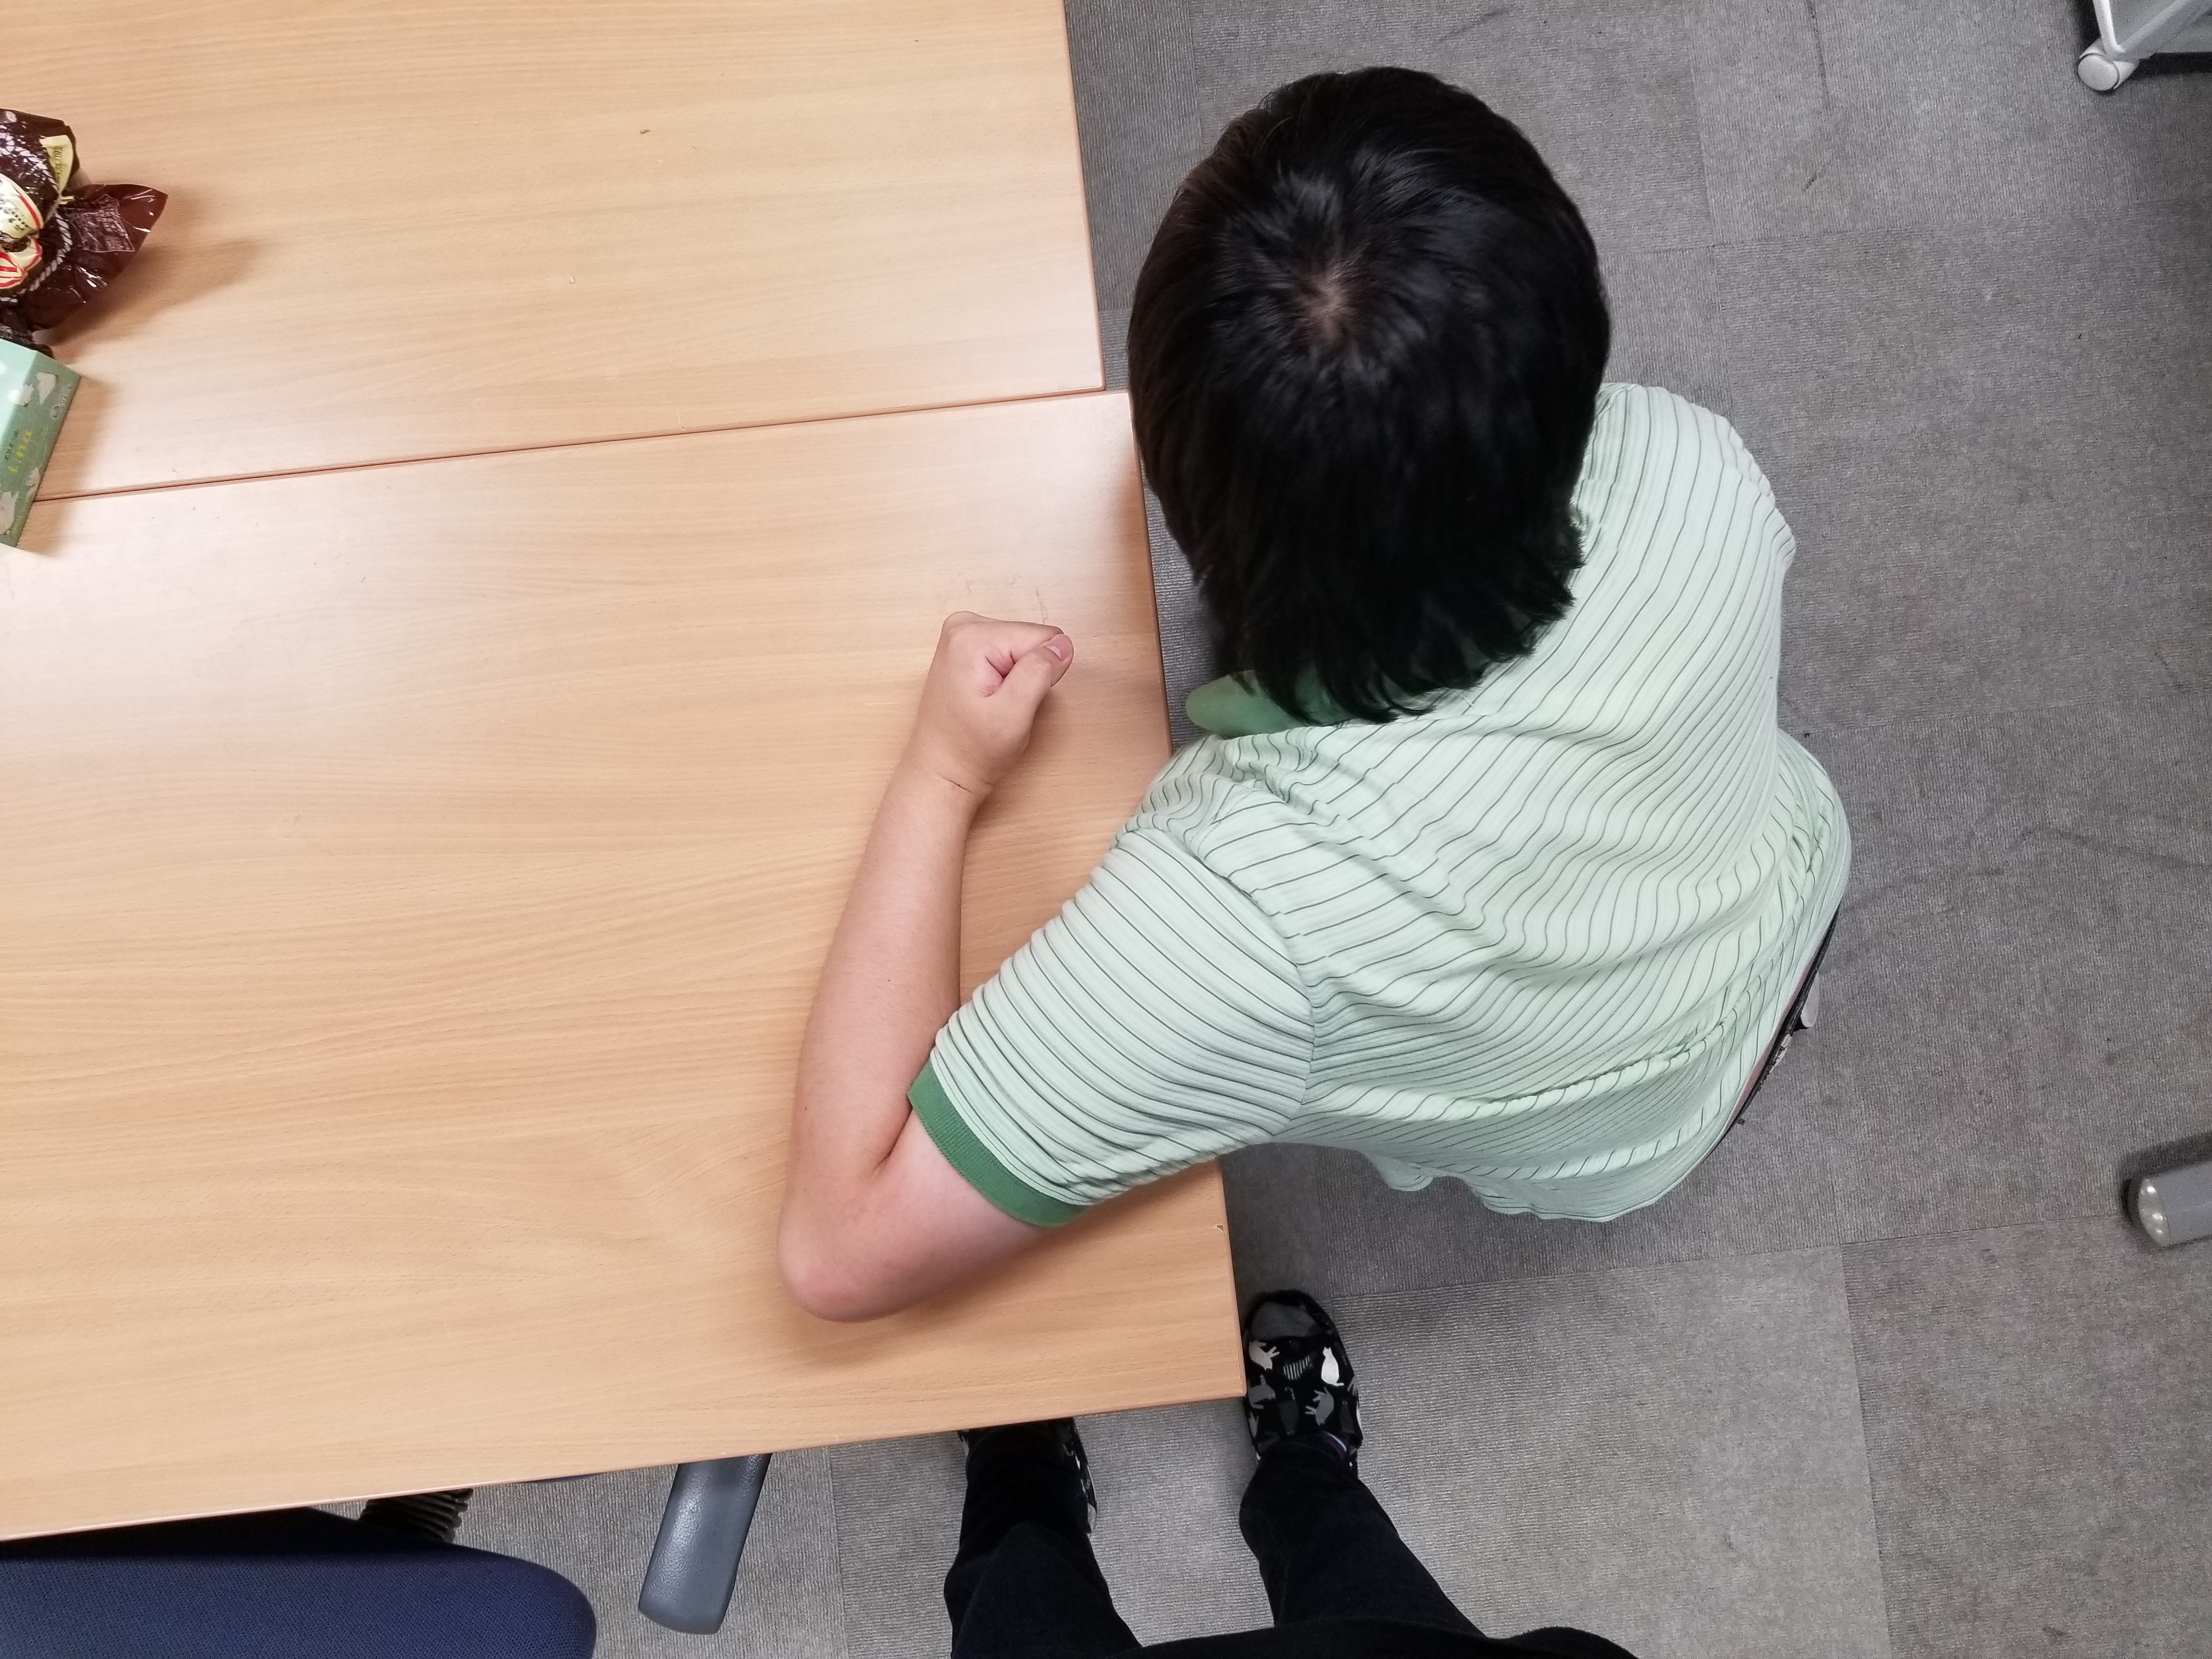
\includegraphics[width=7cm]{images/short.jpg}
    \end{center}
    \caption{腕を縮めた状態}
    \label{fig:short}
  \end{minipage}
  \begin{minipage}{0.5\hsize}
    \begin{center}
      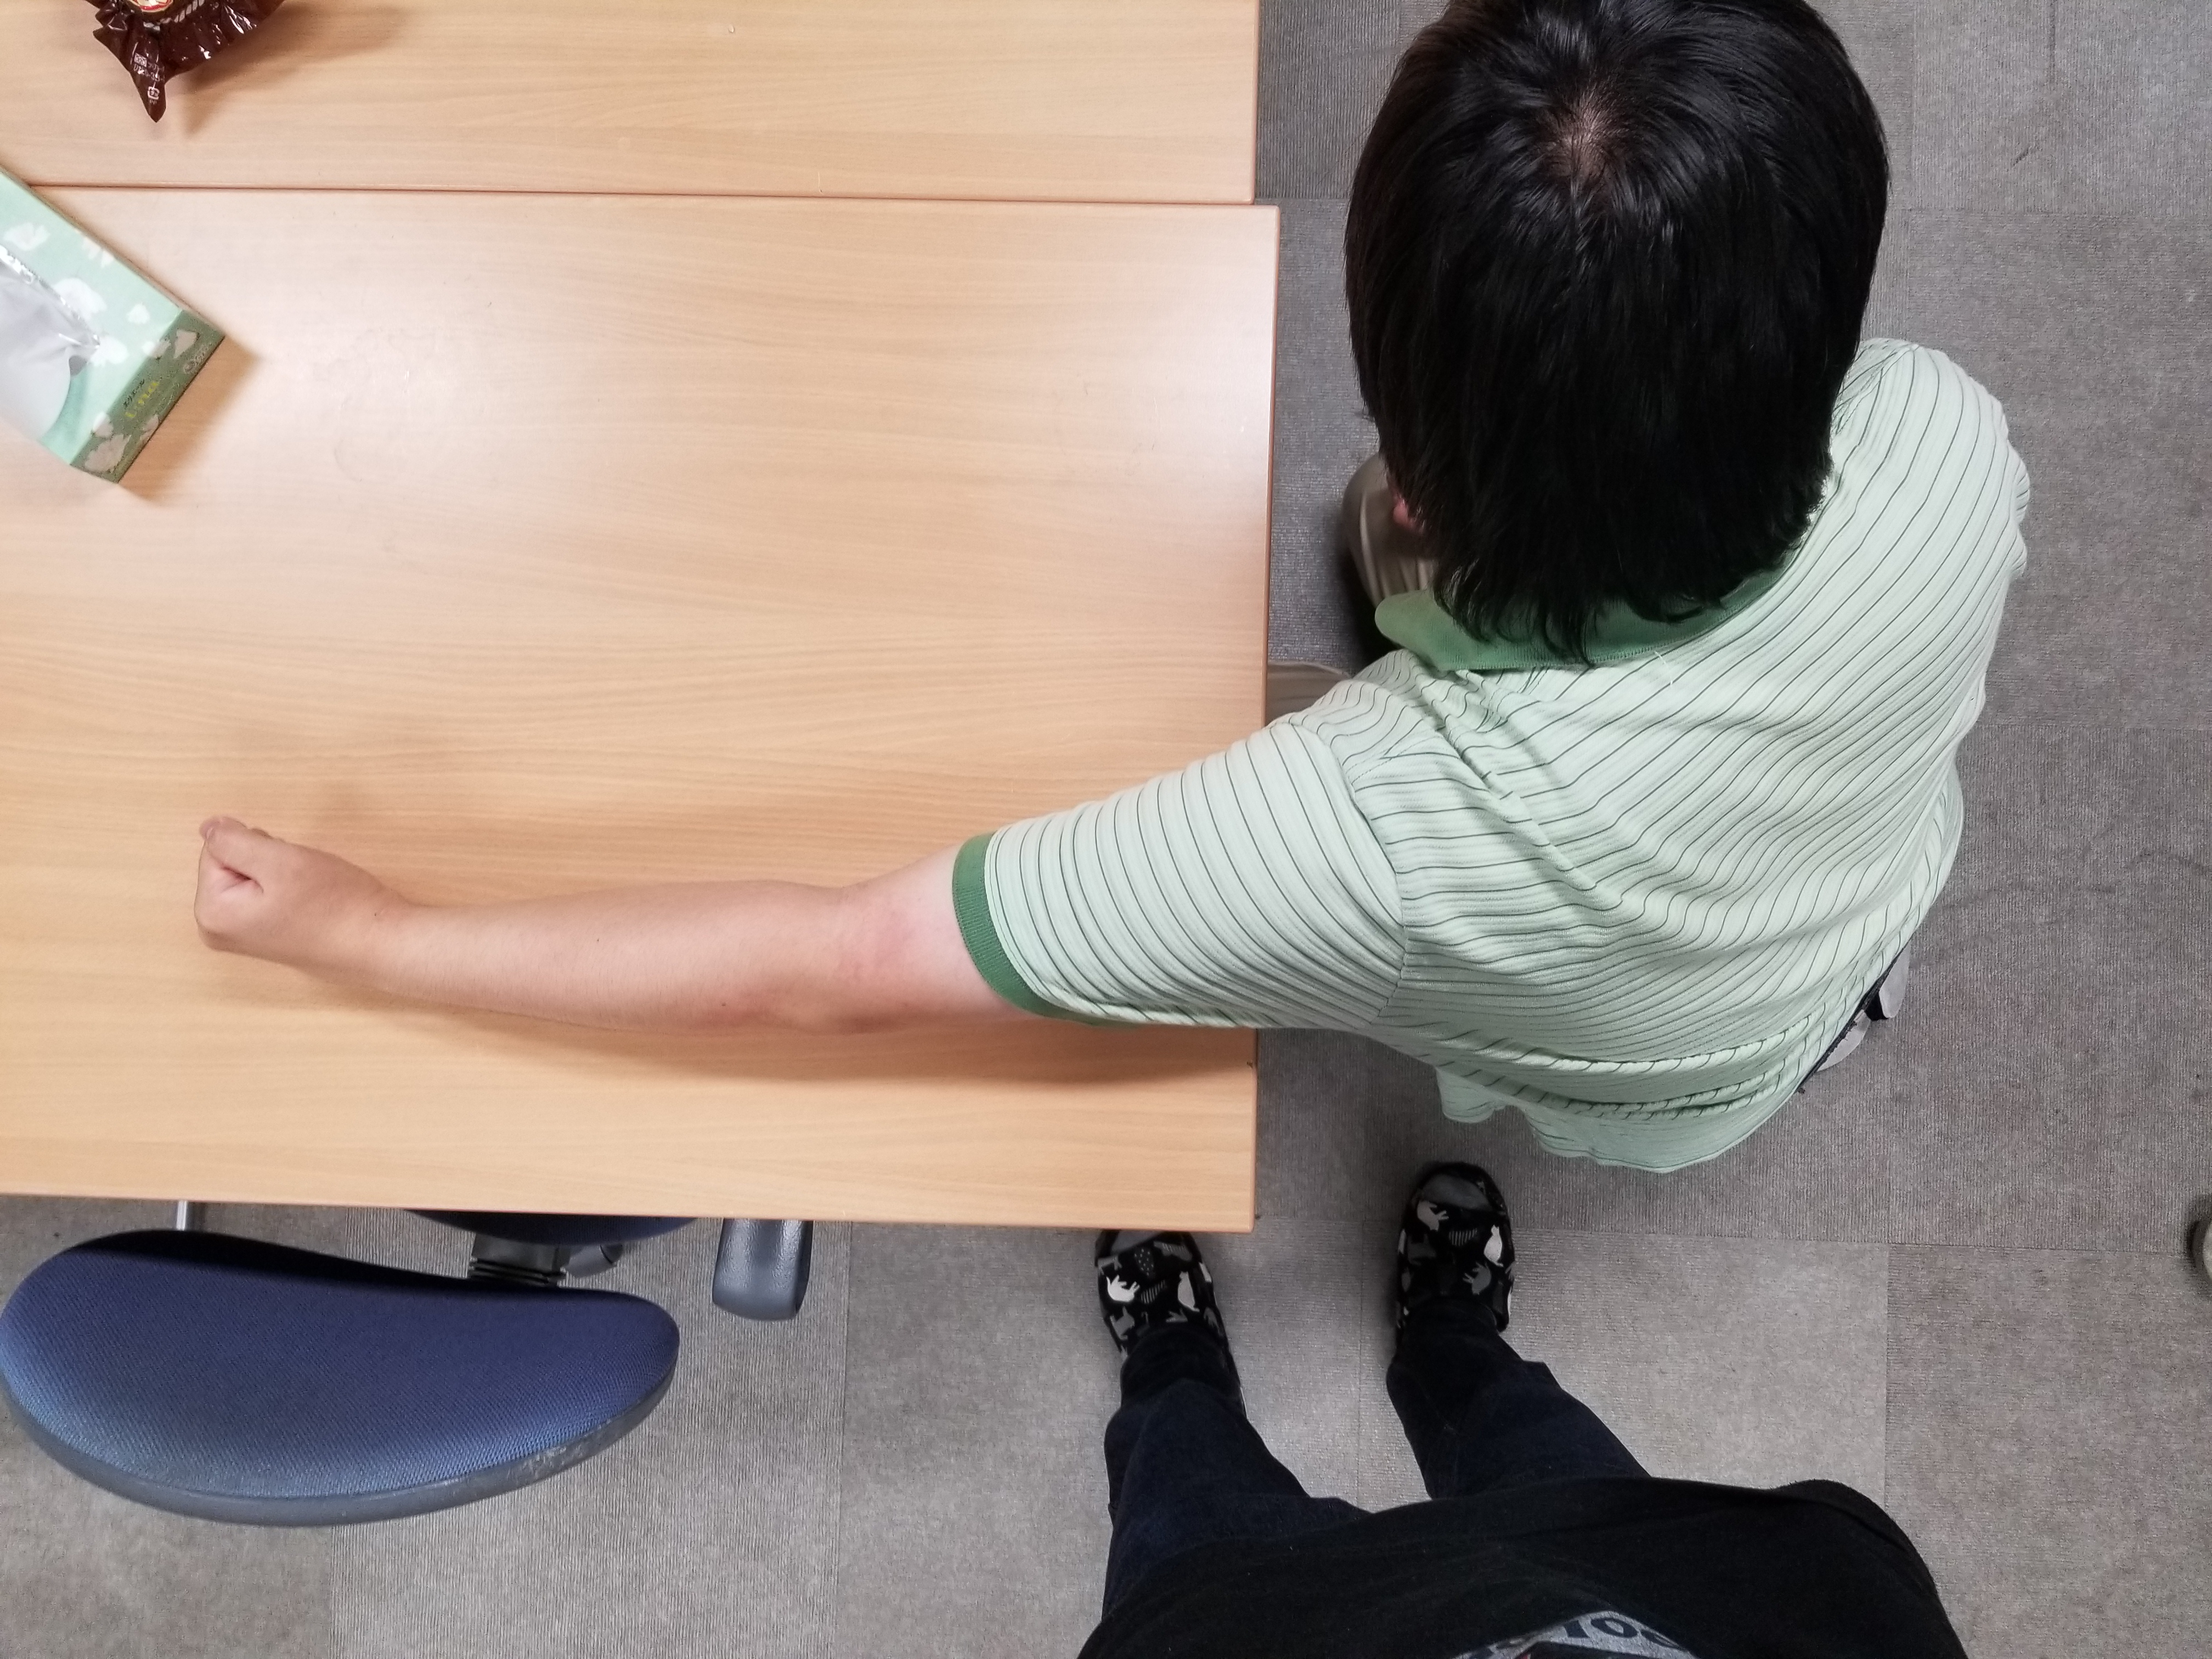
\includegraphics[width=7cm]{images/long.jpg}
    \end{center}
    \caption{腕を伸ばした状態}
    \label{fig:long}
  \end{minipage}
\end{figure}

\subsection{解析}
\subsubsection{筋電位}
筋電位のデータにはいくつかの処理を順番に施して、筋肉の活動度を求めた。
  まずデータから筋電位の特徴を抽出するために、通過帯域を1〜40Hzとしたバンドパスフィルタ(3次バターワース)をかけた。しかし、バンドパスフィルタをかけることによってデータに位相ズレが生じるため、時間軸を反転してもう一度同じフィルタをかけることによってこれを補正した。
  だが見るべきは振幅の変化である。そこでフィルタをかけたデータに整流化と積分を行い、筋肉の活動度を求めた。積分式は以下のものを用いた。この式では、時刻$t$の筋電位$|E(t)|$を$\Delta T$で平均を求めている。
  \begin{equation}
    a(t) = \frac{1}{\Delta T} \int_{t-\frac{\Delta T}{2}}^{t+\frac{\Delta T}{2}} |E(t)| dt
  \end{equation}

\subsubsection{位置座標}
体の位置座標のデータには3つの観測点、そしてそれぞれのx座標とy座標の位置データがある。さらにコマ数やフレーム間隔などの設定上のデータも付随しているため、データをグラフ化しやすくするためにデータの抜き出しをする必要があった。
そこで、位置座標のデータ部分と設定などのそれ以外の部分に分ける、データ部から位置情報を観測点ごとに分けて抜き出す、という二つの処理を行った。
\newpage
\section{結果}
\begin{figure}[h]
  \begin{center}
    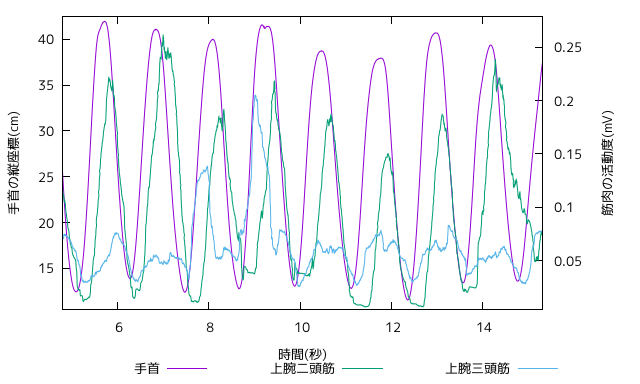
\includegraphics[width=15cm]{images/s1proto.png}
  \end{center}
  \caption{スロー時の運動と筋肉の活動度の関係}
  \label{fig:slow}
\end{figure}
図\ref{fig:slow}は、特に指示を出さず腕を動かしてもらった時のものである。手首の縦方向の座標を第一y軸に、筋肉の活動度を第二y軸に、そして時間をx軸とした。クラフデータは、紫が手首の縦方向の座標、緑が上腕二頭筋の筋肉活動度、青が上腕三頭筋の筋肉活動度を示している。観測点の中では手首の縦方向の座標がもっとも変位が大きく、動きが把握しやすい部分のため、比較のために抜き出した。このグラフでは、見やすくするために時刻5〜15秒の間を拡大表示している。

図\ref{fig:slow}から、例えば時刻10秒の時、腕がもっとも曲げられた状態で伸ばされ始め、少ししてから上腕二頭筋の活動度が大きくなっていっている。そして、伸ばしきったあとある程度腕を曲げたところでその活動度を下げはじめている。これはほとんどの場合において言えることである。またこの時上腕三頭筋は、最大値が上腕二頭筋よりもかなり小さいが、同じような挙動をしている。しかし、いくつかの例においては、腕を伸ばし始めてから伸ばしきるまでの間だけ、上腕二頭筋に匹敵する活動度を見せているものもある。
\newpage
\begin{figure}[h]
  \begin{center}
    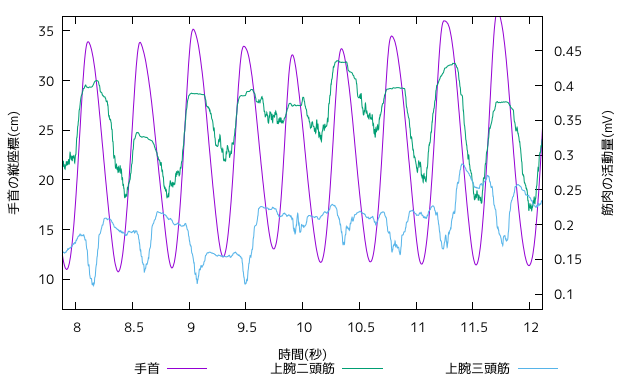
\includegraphics[width=15cm]{images/s2proto.png}
  \end{center}
  \caption{スロー時の運動と筋肉の活動度の関係}
  \label{fig:fast}
\end{figure}
図\label{fig:fast}は、腕を速く動かしてもらった時のものである。軸や凡例は図\ref{fig:slow}と同様である。図\ref{fig:fast}から、例えば時刻8.8秒の時、腕がもっとも曲げられた状態では上腕二頭筋の活動度は低い、この状態から腕が伸ばされ始めると同時に活動度が大きくなっていっている。また腕を曲げるにしたがってその活動度を下げている。要するに手首の縦方向の座標と似たような形である。このとき上腕三頭筋は、腕をもっとも曲げた状態では活動度が大きく、腕が伸ばされるにしたがってその値が小さくなっていっている。これは、上腕二頭筋の位相がずれたような形である。
\section{考察}
私は、上腕二頭筋は腕を縮めるときに、上腕三頭筋は腕を伸ばすときだけに使うものと考えていた。しかし、上腕二頭筋は腕を伸ばすときにも、上腕三頭筋は腕を曲げるときにも、それぞれ使われていることが計測でされた。

人は、片側の筋肉だけでは動作の速度をうまく調整できずに想定した速さより速くなってしまう。そこで、反対側の筋肉(二頭筋なら三頭筋。三頭筋なら二頭筋)を使うことによって移動方向と逆側に力を加えて速さを調整しているのではないだろうか。
そうすれば、伸ばすときに上腕二頭筋を、曲げるときに上腕三頭筋を使っていることの説明ができるだろう。

ところが、動きが遅い時は上腕二頭筋と三頭筋の活動度の起伏がほぼ同じ位置にあり、動きが速い時は起伏の位置が異なっている。けれども、同じ理屈で速さを調整しているのならば起伏の位置は近いものになるはずである。

これは、上腕二頭筋と上腕三頭筋の発達度の違いによって生じた可能性がある。基本的に二頭筋は三頭筋より発達している。ゆっくり動かすときは筋肉はそれほどの活動度を示さないはずだが、二頭筋は三頭筋よりも高い活動度を示すために、三頭筋は二頭筋を抑える必要が出てくる。だから、ゆっくり動かすときは起伏の位置が同じになっているのではないだろうか。
\end{document}